\Chapter{An Introduction to Neutrinos}
\label{Ch1}

    Neutrinos are leptons carrying neutral electrical charge.
    Its neutral lepton nature makes it a fermion that only interacts with other particles through weak interactions.
    From decades of experimental study, it is known that neutrinos come in three flavors, and have antiparticle analogs.
    The neutrino was long assumed to be a massless particle until the discovery of neutrino oscillations, which proved that that at least two of the neutrinos have mass.
    Measurements of neutrino oscillation also showed that neutrino mass eigenstates are not orthogonal with neutrino flavor states, and are significantly mixed with neutrino flavors, in contrast to quark mixing.
    
    Although many theoretical and experimental efforts involved with neutrinos have been completed, the discovery and measurements of neutrinos have brought even more experimental questions into focus: the absolute mass measurement of neutrinos, the observation of lepton CP-violation through neutrino oscillation, probing neutrino-less double beta decay, and the new beyond standard model neutrino states.
    
    Thanks to its rare reaction with other particles, neutrino detection has been applied to aid the research of nuclear and astrophysics.
    Reactor antineutrino detectors are able to remotely monitor a fission reactor's nuclear structure~\cite{bib:DYBSpectrum, bib:DYBEvo}. 
    The neutrino observatory has become an essential component in the multi-messenger astrophysics observations~\cite{bib:IceCube}.

\Section{Beta-decay}
\label{Ch1Sec2}
    
    The study of neutrino physics began with studies of $\beta$-decay.
    During early research on radioactive decay, the process of $\beta$-decay was assumed to be
    \begin{equation}
    (A, Z) \rightarrow (A, Z+1) + e^-.
    \end{equation}
    With energy and momentum conservation, one can easily conclude that reaction should produces a $\beta$ with single kinetic energy.
    In 1914, Chadwick found the energy spectrum of the $\beta$ particle produced from radioactive decay was continuous~\cite{bib:Chadwick}, different from the $\alpha$ and $\gamma$ products that have a sharp distribution.
    Particularly, Ellis and Wooster established the proof of continuous $\beta$ spectrum measurement of $^{210}$Bi~\cite{bib:EandW} shown in Figure~\ref{fig:BiSpectrum}.
    To preserve conservation of energy, in 1932, Pauli postulated the existence of a new particle in his \textit{Open Letter to The Group of Radioactive People at the Gauverein Meeting in Tübingen}, by calling it a ``neutron", as an additional neutral spin-$\frac{1}{2}$ particle produced in $\beta$-decay.

\begin{figure}[h!]
\centering
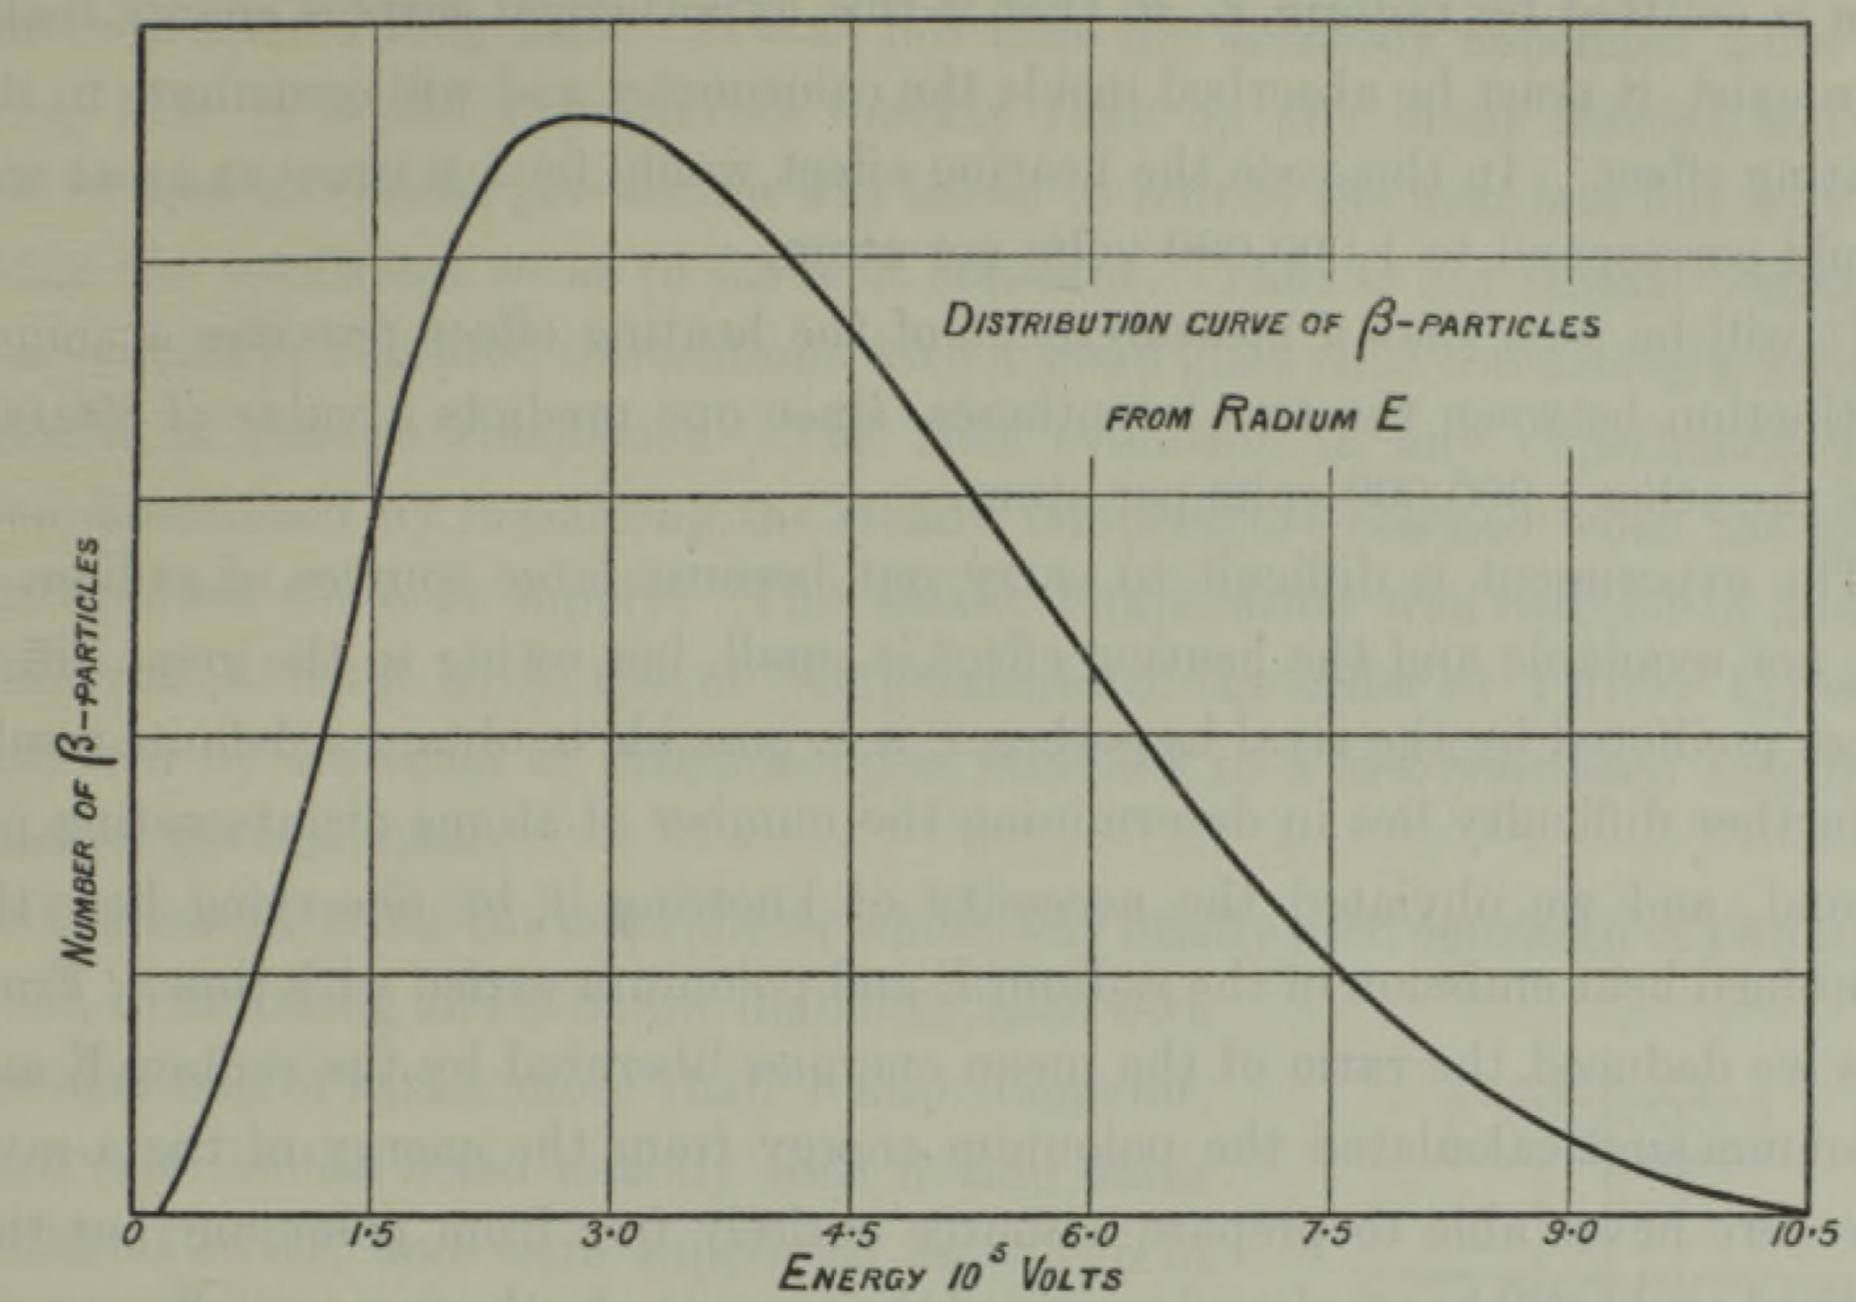
\includegraphics[width=0.6\textwidth]{Figures/BiSpectrum.png}
\caption[The continuous $\beta$ spectrum of $^{210}$Bi]{The continuous $\beta$ energy spectrum measured from $^{210}$Bi $\beta$-decay~\cite{bib:EandW}.}
\label{fig:BiSpectrum}
\end{figure}    
    
    Soon after the discovery of the neutron (the neutral nucleon), Fermi developed his theory of beta decay in 1934~\cite{bib:Fermi}, where the weak interaction was theorized. 
    In Fermi's theory of beta decay, neutrinos were incorporated as a massless daughter particle that carries away a part of the energy of a neutron beta decay:
    \begin{equation}\label{eq1.1}
        n \rightarrow p + e^- + \nu,
    \end{equation}
    where $\nu$ was named as `neutrino' for the first time.
    The neutrino generated in this process was later found to be \nuebar (electron antineutrino) to conserve lepton number in this process.

\Section{The Discovery of Neutrinos}
\label{Ch1Sec2}

    When he proposed the neutrino's existence, Pauli stated they were particles that ``cannot be detected."
    The introduction of the weak interaction meant that neutrinos can interact with other particles by exchanging W or Z bosons.
    Among many types of neutrino-nucleon and -lepton interactions, neutrinos can interact similarly as in $\beta$-decay:
    \begin{equation}
        \label{eq:IBD}
        \nuebar + p \rightarrow n + e^+,
    \end{equation}
    which is named as inverse beta decay (IBD), a quasielastic charged-current (CCQE) reaction between \nuebar and proton mediated by the exchange of a W boson.
    The cross-section of the IBD reaction is
    \begin{equation}
    \label{eq:IBDX}
    \sigma_{IBD} \simeq \frac{G_F^2|V_{ud}^2|}{\pi} (1+3g_A^2)E_\nu^2,
    \end{equation}
    where $G_F$ is the Fermi constant, $V_{ud}$ is the up-down quark mixing magnitude, and the Goldberger–Treiman relation $g_A \simeq 1.27$.
     Equation~\ref{eq:IBDX} estimates the IBD cross-section at the scale of $\sim 10^{-43}\frac{p_eE_e}{\text{MeV}^2}$~(cm$^2$)~\cite{bib:IBDXsection}, where $p_e$ and $E_e$ are momentum and energy of the IBD produced positron.
    Such a rare interaction rate brought a significant challenge in neutrino detection that requires both high neutrino production from the source and a vast amount of protons in the detector.
    
    In 1956, Cowan and Reines discovered neutrinos through the detection of IBD~\cite{bib:CowanReines}.
    The neutrinos detected were \nuebar produced from the $\beta$-decay of daughter isotopes of the nuclear fission reactor at the Savannah River nuclear power plant.
    To detect the IBD signals, two target tanks filled with $^{108}$Cd loaded water were deployed in two gaps made by three vertically aligned liquid scintillator (LS) detectors.
    The signature of the IBD process was the time coincidence between the positron and neutron produced in the reaction.
    When a proton in the water tank was hit by \nuebar, the produced positron annihilated with a electron into a pair of 0.511~MeV $\gamma$, and the neutrons were mostly captured by $^{108}$Cd within 5~\textmu s, emitting capture $\gamma$ rays with total energy from 3~MeV to 10~MeV.
    As they interacted in the LS, the $\gamma$ rays in the LS generate scintillation photons that are eventually collected by the 110 photomultiplier tubes (PMTs) in each LS detector. 
    By detecting $\gamma$ rays from the target tanks with time coincidence, the Cowan and Reines experiment observed 1013 \nuebar events in 900~hours reactor-on data acquisition.
    
    The conservation of lepton flavor requires that $\beta$-decay only produce \nuebar.
    This conservation also forbids interactions like $\overline{\nu}_\mu + p \rightarrow n + e^+$, meaning a ${\nu}_\mu$'s (muon neutrino's) interaction with a nucleon cannot produce an electron~\cite{bib:Ponte1959, bib:Schwartz}.
    In 1962, Schwartz, Lederman, and Steinberger induced high energy $\nu_\mu/\overline{\nu}_\mu$ produced from the decay of the boosted $\pi^\pm$~\cite{bib:numuDiscovery}.
    With a 10~ton spark chamber consisting of 90 aluminum plates, the experiment at Brookhaven National Laboratory was able to distinguish electrons and muons produced from $\nu_\mu/\overline{\nu}_\mu$'s interactions with nucleons. 
    This experiment discovered $\nu_\mu$ by finding that only $\mu^\pm$ were detected in the chamber.
    
    In 2000, the DONUT collaboration at Fermilab discovered $\nu_\tau$ (tau neutrino)  from the decay of boosted $D_s^- \rightarrow \tau^- + \overline{\nu}_\tau$. 
    Since the discovery of $\nu_\tau$, the family of neutrinos in Standard Model has six members: $\nu_e$, $\nu_\mu$, $\nu_\tau$, and their antiparticles.
    
\Section{Observation of Neutrino Oscillations}
    
    Fermi also stated the neutrino should be either massless or extremely light in his study of $\beta$-decay~\cite{bib:Fermi}.
    Following Yang and Lee's discussion of the parity conservation question~\cite{bib:YangLee}, Wu discovered that weak interaction violates parity symmetry by observing $\beta$ momentum direction preference in the $\beta$-decay of polarized $^{60}$Co~\cite{bib:Wu}.
    The parity violation of $\beta$-decay restricts the neutrino helicity to be only left-handed (and antineutrino helicity to be only right-handed).
    Therefore, massless neutrinos and antineutrinos were seemingly preferred in nature to obey the proper representation of the Lorentz group.
    The Standard Model was built with the assumption of massless neutrinos.
    However, the experimental observation of neutrino oscillations proved neutrinos have nonzero masses.

    The research of the oscillating neutrino began from the discovery of the solar neutrino problem. 
    In 1968, Davis \textit{et al.} organized a solar neutrino experiment aiming to detect $\nu_e$ from fusion reactions in the sun~\cite{bib:davis}.
    This experiment used a target containing 390000 liters of C$_2$Cl$_4$ in the Homestake mine to detect the appearance of $^{37}$Ar in the $^{37}$Cl($\nu_e$, $e^-$)$^{37}$Ar reaction.
    The solar neutrino problem arose when the measured flux of $\nu_e$ was found to be one third of that predicted by the Standard Solar Model.
    In the following decades, more solar neutrino flux measurements, including GALLEX~\cite{bib:GALLEX}, GNO~\cite{bib:GNO}, SAGE~\cite{bib:SAGE}, and Kamiokande~\cite{bib:kamioka1996}, observed less solar $\nu_e$ flux than expected.
    Also, atmospheric neutrino measurements from the IMB~\cite{bib:IMB} and Kamiokande~\cite{bib:Kamioka1986} experiments reported fewer atmospheric neutrinos than predicted, which is referred to as the \textit{Atmospheric Neutrino Anomaly}.
    These deficits with respect to theoretical models provided experimental hints of the neutrino oscillation. 
    
    Neutrino oscillation was authoritatively first observed by the Super-K experiment~\cite{bib:SuperK} in 1998. 
    Using a water Cherenkov detector with 50000 tons of pure water and 13000 PMTs, the experiment observed the atmosphere $\nu_\mu$ flux difference among a large range of zenith angles, as shown in Figure~\ref{fig:SuperK}.
    The difference of atmospheric neutrino flux was the result of $\nu_\mu$'s oscillating into other flavors while traveling through the earth prior being collected in the detector.
    
\begin{figure}[h!]
\centering
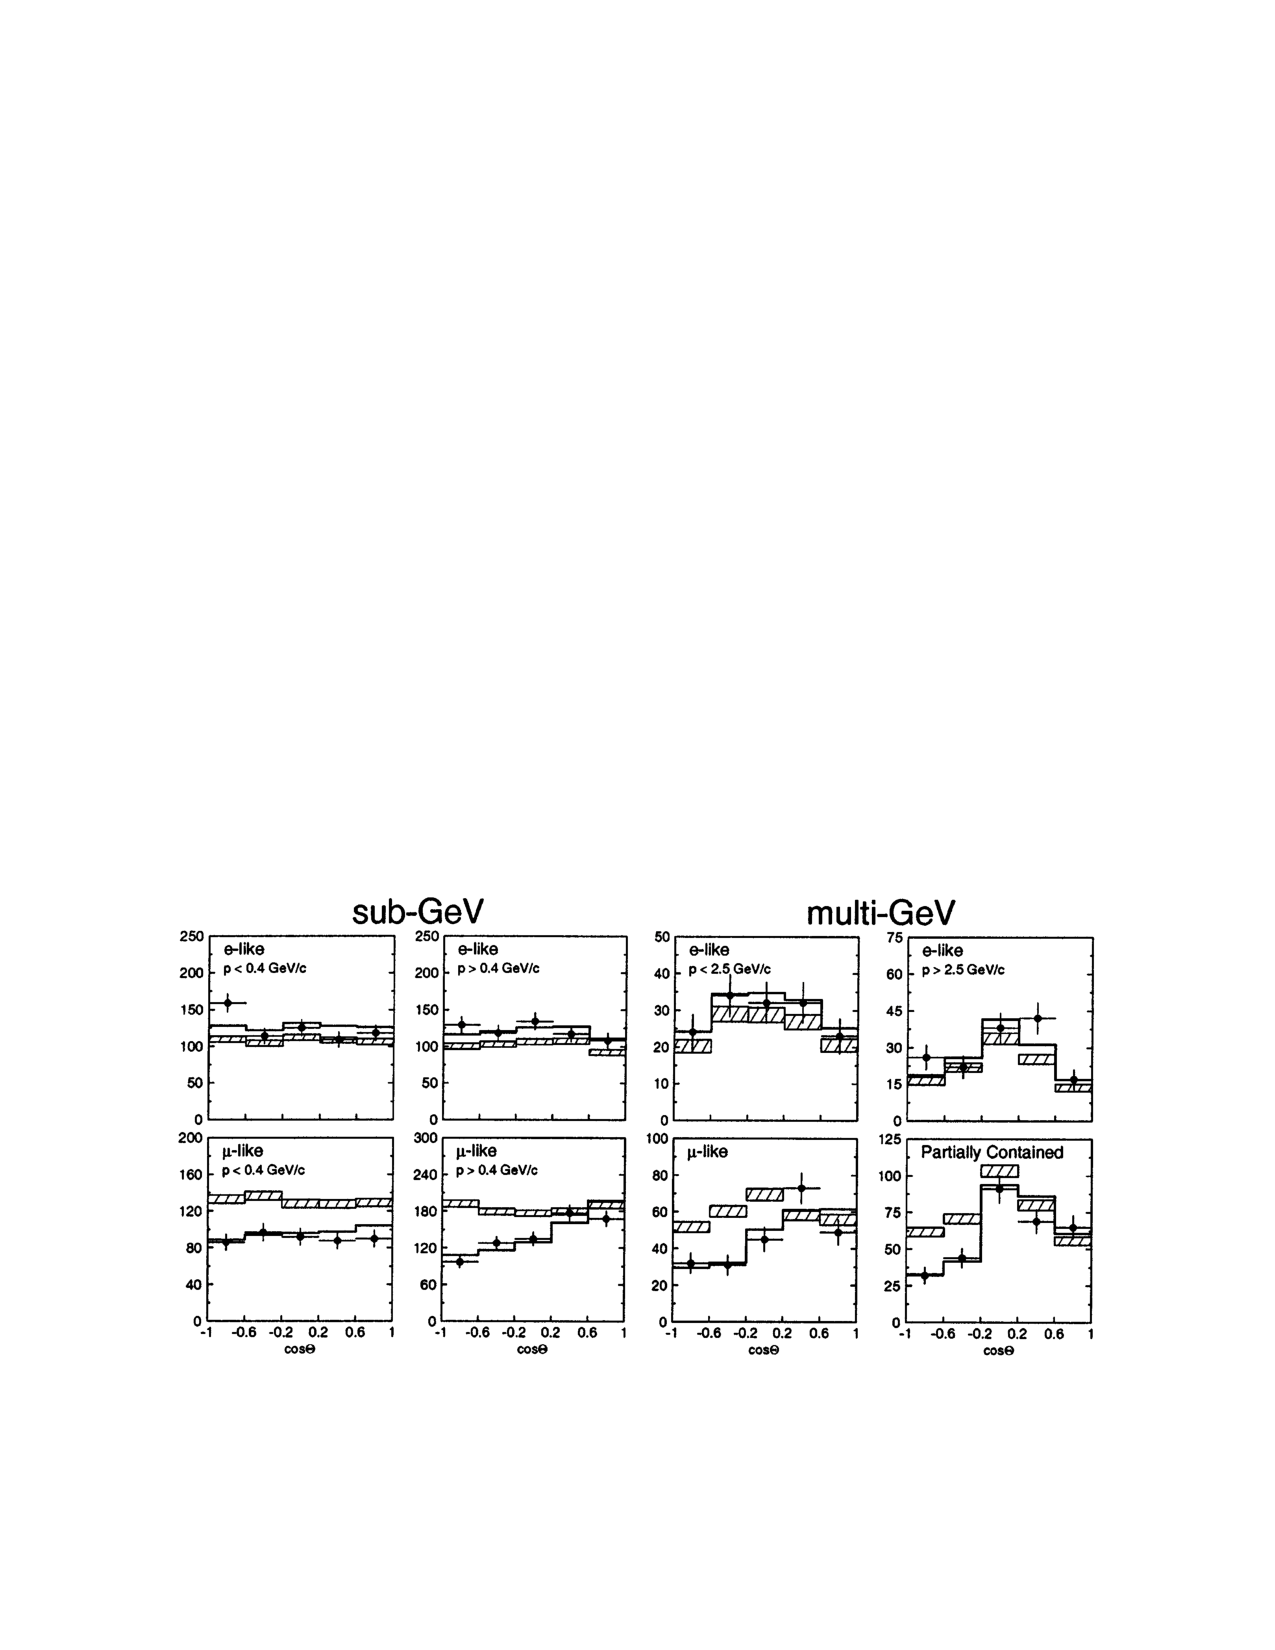
\includegraphics[width=0.95\textwidth]{Figures/SuperK.pdf}
\caption[Atmospheric neutrino oscillation]{The flux of $e$-like and $\mu$-like events measured by the Super-K experiment~\cite{bib:SuperK}. 
The flux of $\mu$-like events, correlated to the number of $\nu_\mu$ collected, varies significantly to zenith angle. 
The solid line (shaded region) represents the Monte-Carlo (MC) simulation with (without) the model of neutrino oscillation.  }
\label{fig:SuperK}
\end{figure}

    In 2001, the SNO experiment~\cite{bib:SNO} deployed a heavy-water Cherenkov detector that was able to detect charged-current (CC), neutral-current (NC) and elastic scattering (ES) to detect solar neutrinos of all flavors in comparison with the $\nu_e$ flux.
    If neutrino oscillates among flavors, the solar $\nu_e$ will oscillates into other flavors while conserving their total flux.
    As shown in Figure~\ref{fig:sno}, the experiment confirmed solar neutrino oscillation by comparing neutrino flux as measured with different scattering modes.
    Super-K and SNO experiments provided substantial experimental evidence of neutrino oscillation and resolved the solar neutrino problem and atmospheric neutrino anomaly.
    
\begin{figure}[h!]
\centering
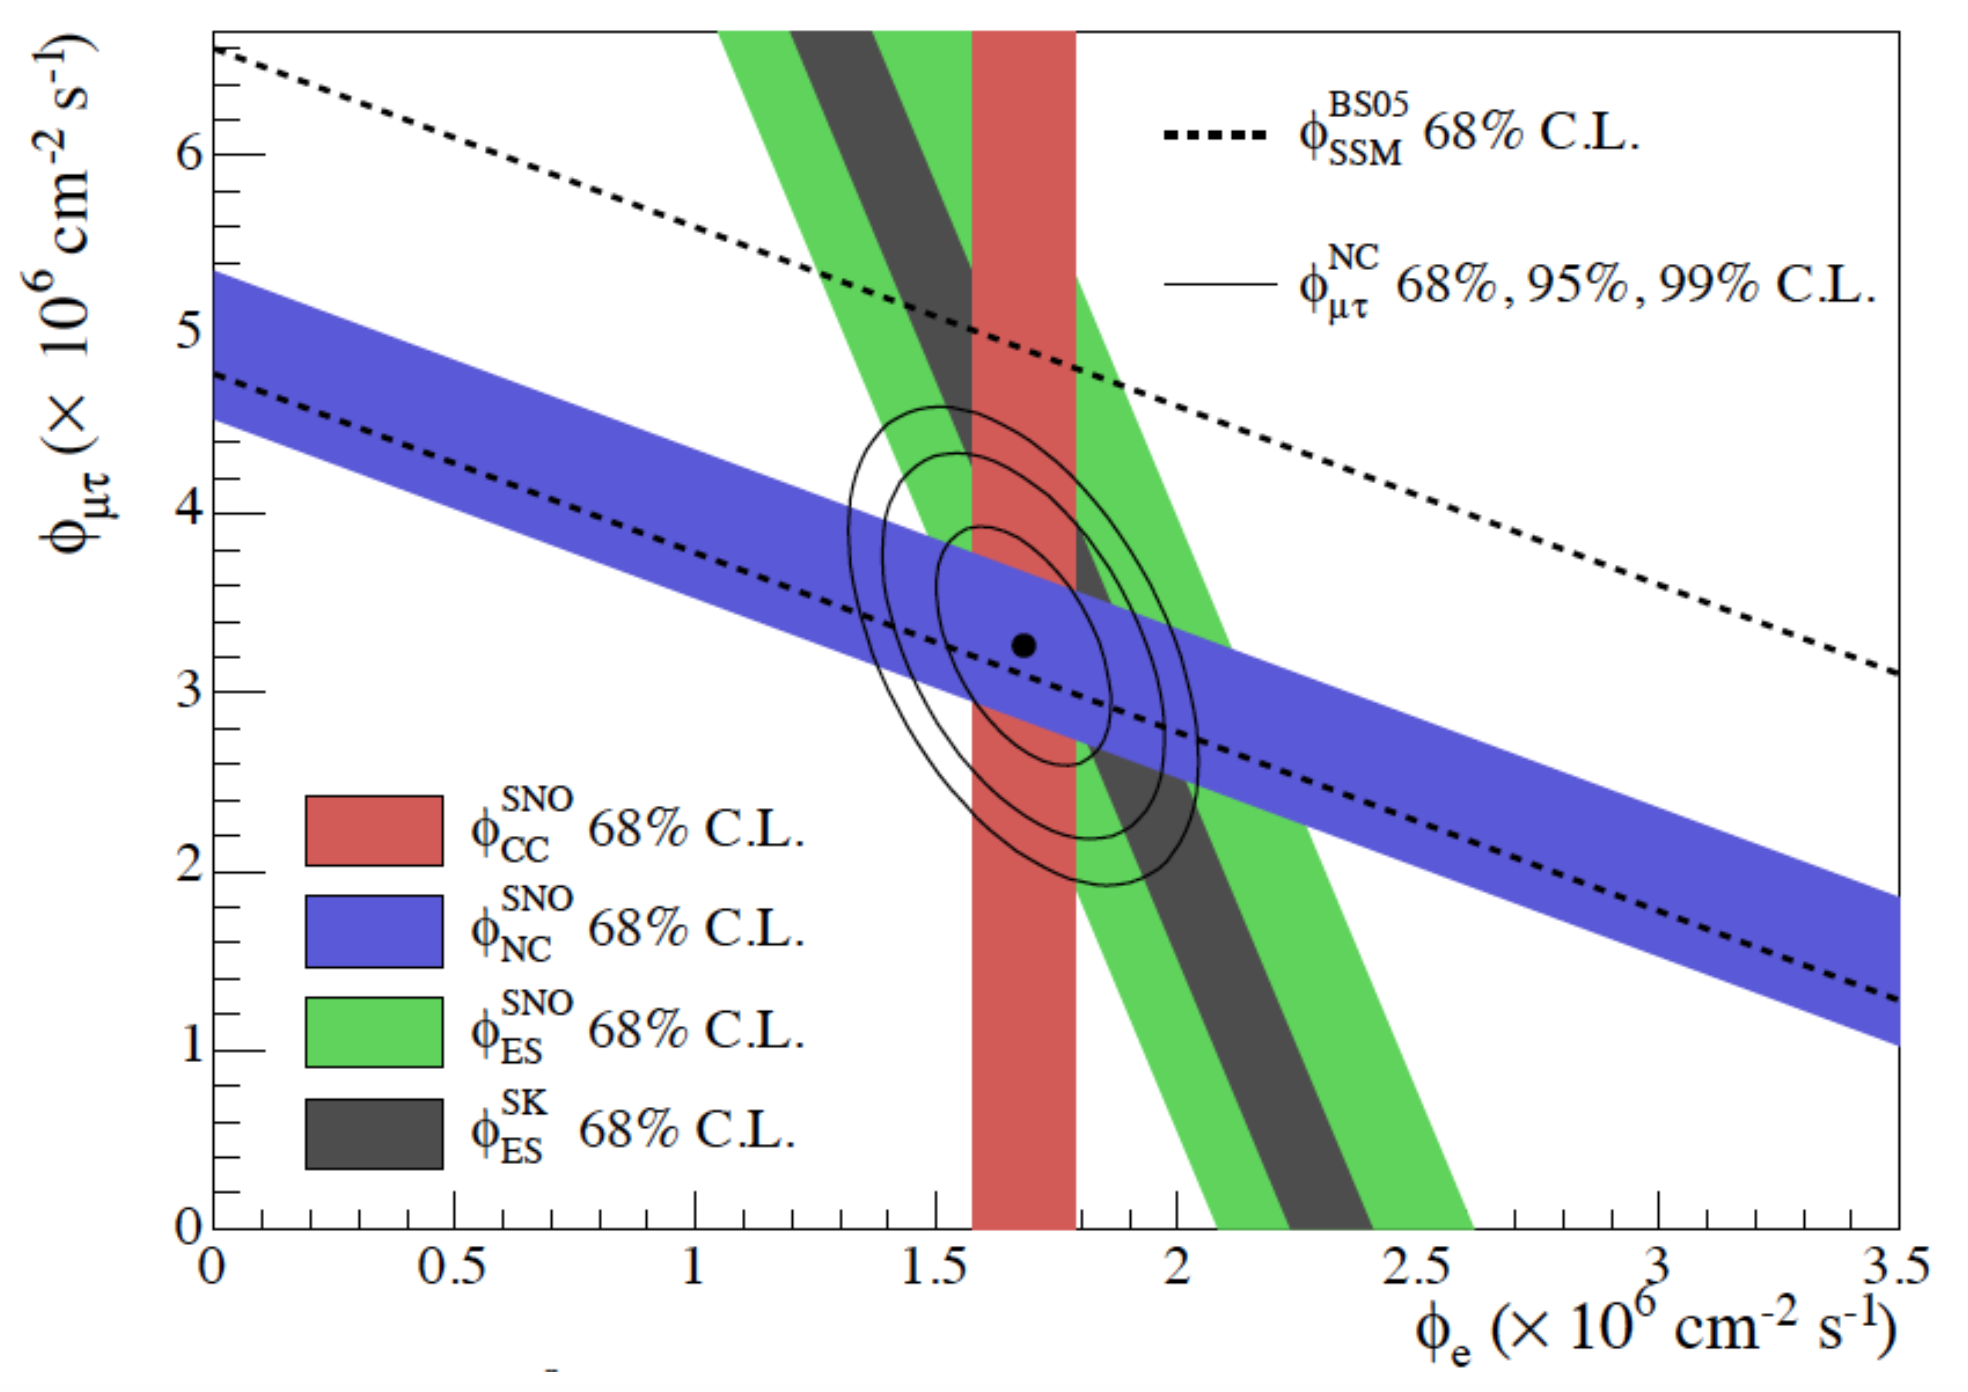
\includegraphics[width=0.6\textwidth]{Figures/sno.png}
\caption[Solar neutrino oscillation]{The flux of different scattering modes of solar neutrinos measured by SNO~\cite{bib:SNO}. The all-flavor flux (NC and ES) agreed. The day-night flux indicates $\nu_e$'s oscillation into other flavors. }
\label{fig:sno}
\end{figure}

\Section{Massive Neutrinos}
    
    The discovery of neutrino oscillation implies that neutrinos have mass.
    Although the natural origin of neutrino mass is undetermined, neutrinos can obtain mass through the Higgs mechanism similar to other leptons. 
    Under the assumption of the neutrino being Dirac fermion (particle distinct from antiparticle), a Higgs-lepton Yukawa Lagragian term can be expressed as
\begin{equation}\label{eq4}
\mathscr{L}_H = -\left(\frac{v+H}{\sqrt{2}}\right)\left[\overline{l'_L}Y'^{l}l'_R +\overline{\nu'_L}Y'^{\nu}\nu'_R\right],
\end{equation}
    where $v$ is the Higgs vacuum expectation value (VEV), $H$ is the Higgs field, and $Y$ is the Yukawa coupling matrix. 
    The matrix can be diagonalized with the unitary matrices $V_L$ and $V_R$.
\begin{equation}\label{eq5}
V^\dagger_LY'V_R = Y,\   \ \textrm{with} \   \ Y_{kj} = y_k\delta_{kj} \   \ (k,j = 1,2,3),
\end{equation}
    where $y_k$ is the eigenvalue of Yukawa coupling matrix. The three-generation neutrino mass mixing is defined as:
\begin{equation}\label{eq6}
\nu'_L \rightarrow V^{\nu\dagger}_L\nu'_L = \left( \begin{array}{c}
\nu_{1L} \\
\nu_{2L} \\
\nu_{3L} \\
\end{array} \right) \   \ \text{and} \   \ \nu'_R \rightarrow V^{\nu\dagger}_R\nu'_R = \left( \begin{array}{c}
\nu_{1R} \\
\nu_{2R} \\
\nu_{3R} \\
\end{array} \right).
\end{equation}
    Considering $l_\alpha = l_{\alpha L} + l_{\alpha R}$ and $\nu_k = \nu_{kL} + \nu_{kR}$, the Lagrangian can be rewritten as
\begin{equation}\label{eq7}
\begin{aligned}
\mathscr{L}_H & = -\left(\frac{v+H}{\sqrt{2}}\right)\left[ \sum\limits_{\alpha = e, \mu, \tau} y_{\alpha}^l\overline{l_{\alpha L}}l_{\alpha R} + \sum\limits_{k = 1, 2, 3}y_k^\nu \overline{\nu_{kL}}\nu_{kR} \right] \\
& = - \sum\limits_{\alpha = e, \mu, \tau} \frac{y_\alpha^l v}{\sqrt{2}}\overline{l_{\alpha}}l_{\alpha} - \sum\limits_{k = 1, 2, 3} \frac{y_k^\nu v}{\sqrt{2}} \overline{\nu_{k}}\nu_{k} - \sum\limits_{\alpha = e, \mu, \tau} \frac{y_\alpha^l}{\sqrt{2}}\overline{l_{\alpha}}l_{\alpha}H - \sum\limits_{k = 1, 2, 3} \frac{y_k^\nu}{\sqrt{2}} \overline{\nu_{k}}\nu_{k}H.
\end{aligned}
\end{equation}
    Since $\nu_k = \nu_{kL} + \nu_{kR}$, the Dirac mass term of neutrino is simplified as
\begin{equation}\label{eq8}
\begin{aligned}
    \mathscr{L}^D_{mass} &= -\sum\limits_{k = 1, 2, 3} m_k^D\overline{\nu_{k}}\nu_{k} + \textrm{H.c.} \\
    & = -\sum\limits_{k = 1, 2, 3}m_k^D(\overline{\nu_{kL}}\nu_{kR} + \overline{\nu_{kR}}\nu_{kL}) + \textrm{H.c.},
\end{aligned}
\end{equation}
    where the Dirac mass of the neutrino $m_k^D = \frac{y_k^\nu v}{\sqrt{2}}$ and $\overline{\nu_{kL}}\nu_{kL} = \overline{\nu_{kR}}\nu_{kR} = 0$.
    This mechanism for neutrinos to obtain mass involves a right-handed neutrino $\nu_R$, also referred to as the \textit{sterile neutrino} for its incapability of interacting under the parity-violating weak force.
    
    Because of its neutral nature, neutrinos are also candidates to be Majorana fermions (the particles being the antiparticles of themselves).
    Under this condition, the neutrino field is
    \begin{equation}\label{eq9}
        \nu = \nu_L + \mathcal{C}\overline{\nu_L}^T,
    \end{equation}
    where neutrino $\mathcal{C}$ is a charge conjugate matrix.
    The Majorana mass term of the lepton Lagrangian can be written as 
    \begin{equation}\label{eq10}
\begin{aligned}
    \mathscr{L}^M_{mass} &= \frac{1}{2}m_L{\nu_{L}^T} \mathcal{C}^\dagger \nu_{L} + \textrm{H.c.},
\end{aligned}
\end{equation}
    in which $m^L$ is the left-handed Majorana mass.
    The Majorana mass term of neutrino avoids the assumption of a right handed neutrino.
    
    However, it is theoretically allowed that both right handed neutrinos and Majorana neutrinos exist. 
    In this case, a more general neutrino mass term for single neutrino scenario is defined as 
    \begin{equation}
    \label{eq11}
    \begin{aligned}
    \mathscr{L}_{mass}^{D+M} &= - m_D(\overline{\nu_{L}}\nu_{R} + \overline{\nu_{R}}\nu_{L}) + \frac{1}{2}m_L{\nu_{L}^T} \mathcal{C}^\dagger \nu_{L} + \frac{1}{2}m_R{\nu_{R}^T} \mathcal{C}^\dagger \nu_{R} + \textrm{H.c.} \\
    & = \frac{1}{2}(\begin{array}{cc}
    \overline{\nu^C_L} & \overline{\nu_R} \end{array}) 
    \left(\begin{array}{cc}
    m_L & m_D \\
    m_D & m_R
    \end{array}\right)
    \left(\begin{array}{c}
    \nu_L \\
    \nu_R^C
    \end{array}\right) + \textrm{H.c.}.
    \end{aligned}
    \end{equation}
    In a special case, when $m^D \ll m_R$ and $m_L = 0$, Equation~\ref{eq11} can be diagonalized as
    \begin{equation}
    \label{eq12}
    \mathscr{L}_{mass}^{D+M}  = \frac{1}{2}(\begin{array}{cc}
    \overline{\nu_1} & \overline{\nu_2} \end{array}) 
    \left(\begin{array}{cc}
    \frac{m_D^2}{m_R} &  \\
     & m_R
    \end{array}\right)
    \left(\begin{array}{c}
    \nu_1 \\
    \nu_2
    \end{array}\right) + \textrm{H.c.}
    \end{equation}
    This is called the Type-I seesaw mechanism, a possible explanation of the tiny mass of the left-handed neutrino~\cite{bib:yanagida, bib:Ramond}.

\Section{Theory of Neutrino Oscillation}
    
    The theoretical study of neutrino oscillations started in the 1950s.
    Pontecorvo~\cite{bib:Pontecorvo1957, bib:Pontecorvo1957qd} proposed neutrino oscillation inspired by observation of $K^0 \leftrightarrow \overline{K}^0$ oscillations.
    In 1967, Maki, Nakagawa, and Sakata discussed the theory of two-neutrino flavor mixing~\cite{bib:Maki1962}.
    Later in 1969, Gribov and Pontecorvo explicitly developed the theory of neutrino oscillation with mass state mixing~\cite{bib:GRIBOV1969}. 
    For massive neutrinos, the neutrino portion of the Lagrangian can be expressed analogously to other massive particles:
\begin{equation}
\label{eq13}
\mathscr{L}_\nu = -\left[m^\nu_\alpha\overline{\nu_\alpha}\nu_\alpha + m^\nu_\beta\overline{\nu_\beta}\nu_\beta + m^\nu_\alpha m^\nu_\beta(\overline{\nu_\alpha}\nu_\beta + \overline{\nu_\beta}\nu_\alpha) \right] \   \ (\alpha, \beta = e, \mu, \tau).
\end{equation}
    This equation can be rewritten as
\begin{equation}
\label{eq14}
\mathscr{L}_\nu = \overline{\nu}_\alpha\mathcal{M}^\nu\nu_\beta.
\end{equation}
    where the $\mathcal{M}'^\nu$ can be diagonalized. 
    The conversion between the two matrix expressions above transforms the flavor states of neutrinos to mass states by a unitary matrix $U$:
\begin{equation}\label{eq15}
\left(\begin{array}{c}
\nu_\alpha \\
\nu_\beta
\end{array}\right) = \left(\begin{array}{cc}
\cos\theta & \sin\theta \\
-\sin\theta & \cos\theta
\end{array}\right)\left(\begin{array}{c}
\nu_k \\
\nu_l
\end{array}\right).
\end{equation}

    When $\theta \neq 0$, this transformation is a two generation mixing of neutrino mass eigenstates and neutrino flavors, meaning a neutrino's flavor is not orthogonal to its mass eigenstates.
    This matrix can be expanded to three neutrino mixing with the unitary matrix $U_{PMNS}$, the Pontecorvo-Maki-Nakagawa-Sakata (PMNS) matrix, a neutrino equivalent to the CKM mixing matrix of the quark sector. 
    In addition to the 3x3 angular transformation, this matrix also includes a CP-violation phase factor $\delta_{CP}$ and a diagonal mixing matrix of Majorana neutrino terms $D_\textrm{Majorana}$, where $\xi_1$ and $\xi_2$ are Majorana phase terms. 
    The three generation neutrino mixing matrix is 
    \begin{equation}\label{eq16}
    \begin{aligned}
    U & =  U_{PMNS}\cdot D_\textrm{Majorana} \\
    & =  \left(\begin{array}{ccc}
    U_{e1} & U_{e2} & U_{e3} \\
    U_{\mu 1} & U_{\mu 2} & U_{\mu 3} \\
    U_{\tau 1} & U_{\tau 2} & U_{\tau 3}
    \end{array}\right) \\
    & = \left(\begin{array}{ccc}
    1   &   &  \\
        &   c_{23}  & s_{23} \\
        &   -s_{23} & c_{23}
    \end{array}\right) 
    \left(\begin{array}{ccc}
    c_{13}  &   & s_{13}e^{-i\delta_{CP}} \\
        & 1 &  \\
    -s_{13}e^{i\delta_{CP}}  &   & c_{13}
    \end{array}\right) 
    \left(\begin{array}{ccc}
    c_{12}  & s_{12}  &  \\
    -s_{12} & c_{12} &  \\
        &   & 1
    \end{array}\right)  \\
    &\cdot\left( \begin{array}{ccc}
    e^{i\xi_1/2} & & \\
    & e^{i\xi_2/2} & \\
    & & 1 \\
    \end{array}\right),
    \end{aligned}
    \end{equation}
    where $s_{ij} = \sin\theta_{ij}$ and  $c_{ij} = \cos\theta_{ij}$.

    Hence, the flavor eigenstates of the neutrino can be described as a sum of the mass states with a matrix element form $U_{PMNS}$:
    \begin{equation}\label{eq17}
    |\nu_\alpha\rangle = \sum\limits_{k=1,2,3} U^*_{\alpha k}|\nu_k\rangle.
    \end{equation}
    Using the time-dependent Schr{\"o}dinger equation, the time evolution of neutrino flavor is expressed as
    \begin{equation}
    \label{eq18}
    |\nu_\alpha(t)\rangle = \sum\limits_{k=1,2,3} U^*_{\alpha k}e^{-i(E_k)t}|\nu_k\rangle.
    \end{equation}
    Therefore, the probability of a neutrino oscillating from one flavor to the other is
    \begin{equation}\label{eq19}
    \begin{aligned}
    P_{\nu_\alpha\rightarrow\nu_\beta} & =|\langle\nu_\beta|\nu_\alpha(t)\rangle|^2 \\
    & =\sum\limits_{k,j}U^*_{\alpha k} U_{\beta k} U_{\alpha j} U^*_{\beta j} e^{-i(E_k-E_j)t} \\
    & =\sum\limits_{k,j}U^*_{\alpha k} U_{\beta k} U_{\alpha j} U^*_{\beta j}\exp\left(-i\frac{\Delta m^2_{kj}L}{2E}\right),
    \end{aligned}
    \end{equation}
    where $\Delta m_{kj}^2 =m_k^2 - m_j^2$, $L$ is the neutrino travelling distance, and $E$ is the kinetic energy of the neutrino.
    This equation proves that a nonzero neutrino oscillation probability requires the mixing of massive neutrinos.
    It also shows that the phase of the neutrino oscillation depends on the factor $\frac{\Delta m^2_{kj}L}{2E}$, resolving both the solar neutrino problem and the atmospheric neutrino anomaly. 
    
    The probability shown in Equation~\ref{eq19} can be generalized to any neutrino flavor transition in oscillation as
\begin{equation}\label{eq20}
\begin{aligned}
    P_{\nu_\alpha\rightarrow\nu_\beta} = \delta_{\alpha\beta} & -  4 \sum\limits_{k>j}\textbf{Re} \left[ U^*_{\alpha k} U_{\beta k} U_{\alpha j} U^*_{\beta j}\right]\sin^2\left(\frac{\Delta m^2_{kj}L}{4E}\right) \\
     & \pm 2 \sum\limits_{k>j} \textbf{Im} \left[
     U^*_{\alpha k} U_{\beta k} U_{\alpha j} U^*_{\beta j}\right]\sin\left(-i\frac{\Delta m^2_{kj}L}{2E}\right).
\end{aligned}
\end{equation}
    The imaginary component is positive for neutrinos and negative for antineutrinos. 
    In two neutrino mixing, Equation~\ref{eq19} can be simplified as
    \begin{equation}\label{eq21}
    \begin{aligned}
    P_{\nu_\alpha\rightarrow\nu_\beta} & = \sin^2{2\theta}\sin^2\left( 1.27\frac{\Delta m^2L}{E} \right)
    \end{aligned}
    \end{equation}
    to calculate the appearance probability of one flavor during neutrino oscillation in vacuum.
    Similarly, the survival probability of the original neutrino flavor can be written as 
    \begin{equation}\label{eq22}
    \begin{aligned}
    P_{\nu_\alpha\rightarrow\nu_\alpha} & = 1- \sin^2{2\theta}\sin^2\left( 1.27\frac{\Delta m^2L}{E} \right).
    \end{aligned}
    \end{equation}
    The probability Equations \ref{eq21} and \ref{eq22} are frequently used as a theoretical tool in neutrino oscillation experiments to calculate expected levels of oscillation.

\Section{Measurements of Neutrino Oscillation}
    
    Experimental efforts have been made in the past two decades to determine the key neutrino oscillation parameters.
    By measuring the flux of disappeared or appeared neutrinos at various baselines, experiments have been able to measure the oscillation parameters, including $\theta_{23}$, $\theta_{13}$, $\theta_{12}$, $\Delta m^2_{21}$, and $|\Delta m^2_{31}|$. 
    $\theta_{12}$ and $\Delta m^2_{21}$ were determined by the  phenomenological analyses of solar neutrino flux measurements~\cite{bib:SNOPRC} and KamLAND reactor \nuebar oscillation measurement~\cite{bib:KamLAND03}.
    By measuring the disappearance of $\nu_\mu$ and $\overline{\nu}_\mu$ in atmospheric neutrino experiments~\cite{bib:MACRO,bib:Soudan2}, long baseline accelerator neutrino experiments~\cite{bib:k2k,bib:MINOS,bib:t2k,bib:nova}, and neutrino telescope observation~\cite{bib:ANTARES, bib:ICEosc}, $\theta_{23}$ and $|\Delta m^2_{31(32)}|$ have been measured.
    $\theta_{13}$ has been thoroughly measured in $\sim$1~km scale baseline reactor $\nuebar$ flux measurements~\cite{bib:DYBosc,bib:RENO,bib:DBChooz}.
    The current preferred neutrino mass mixing parameters are listed in Table~\ref{tab:1.1}.
    \begin{table}[h]
    \centering
    \caption[Key parameters of neutrino oscillation]{Measured parameters of neutrino oscillation~\cite{bib:PDG}.}
    \begin{tabular}{lll}
    \hline
    \hline
    Parameters                  & Value             & 3-$\sigma$    \\ \hline
    $\sin^2(\theta _{12})$      & 0.297             & $0.250 - 0.354$
    \\ \hline
    $\sin^2(\theta _{23})$      & 0.425 (normal)    & $0.381 - 0.615$ \\
                                & 0.589 (inverted)  & $0.384 - 0.636$ \\ \hline
    $\sin^2(\theta_{13})$       & 0.0215 (normal)   & $0.0190 - 0.0240$ \\   
                                & 0.0216 (inverted) & $0.0190 - 0.0242$ \\ \hline
    $\Delta m^ 2_{21} (10^{-5}\textrm{eV}^2) $      & 7.57              & $6.93 - 7.96$ \\ \hline
    $|\Delta m^ 2_{31}| (10^{-3}\textrm{eV}^2) $    & 2.56 (normal)     & $2.45 - 2.69$\\
                                & 2.54 (inverted)   & $2.42 - 2.66$\\
    \hline
    \end{tabular}
    \label{tab:1.1}
    \end{table}
    where ``normal" and ``inverted" represents the two untested assumptions of the neutrino mass hierarchy. 
    \textit{Normal hierarchy} suggests $\nu_1 < \nu_2 < \nu_3$ in mass. 
    \textit{Inverted hierarchy} suggests $\nu_3 < \nu_1 < \nu_2$ in mass. 
    
\Section{Future Tasks of Neutrino Experiments}
\label{ch1sec7}
    
    The properties of massive neutrinos are of primary interest for future experimental research, as they are the first solid experimental evidence of physics beyond the Standard Model.  
    Studies of the Dirac or Majorana nature of neutrinos are conducted worldwide. 
    If neutrinoless double $\beta$-decay ($0\nu\beta\beta$) is observed, neutrinos can be determined as the first Majorana fermion ever detected.
    Several experiments are directly measuring the neutrino mass by searching the upper limit of $\beta$ spectra from specific isotopes with very high energy resolution. 
    
    To resolve the neutrino mass hierarchy, observe leptonic CP violation, and search the light sterile neutrino, more precise measurements of neutrino oscillations from different sources at various baselines are needed. 
    These studies involve precise measurement of different transition ratios in oscillation, high-resolution energy spectrum measurement, neutrino-antineutrino oscillation difference, and very short baseline oscillation measurements.